% quiz
% - H1 reduction of order solving for general sol.
% - H3 find general sol. by method of undetermined coeff.
% - H4 find general sol.(?) by variation of parameters

\chapter{Differential Equations}

A \textit{differential equation} is an equation involving a quantity and one or more of its derivatives.

\section*{1 Ordinary Differential Equations}

An ODE involves the derivative of the dependent variable with respect to a single independent variable.

\subsection{Solving by Integration}

\begin{definition}[Solution to a differential equation] A function $y = f(x)$ that satisfies the differential equation when $f$ and its derivatives are substituted into the equation.
\end{definition}

% \begin{procedure}[Making a direction field] This procedure can be used to approximately graph a differential equation, even if an explicit solution cannot be found.
  
%   Factor the equation in terms of $y' = f'(x)$. At each $x,y$-value on a grid of a graph, evaluate $y'$ and draw a short line with the slope $y'$ at the $x,y$-value.
% \end{procedure}

\begin{procedure}[Euler's Method] To numerically approximates the solution to the differential equation $y' = F(x, y)$ with $y(x_0) = y_0$,
  \[
    y_n = y_{n - 1} + F(x_{n-1}, y_{n - 1})(x_n - x_{n - 1})
  \]
\end{procedure}

\begin{definition}[Separable Equation] A separable equation is a differential equation where
  \[
    \frac{dy}{dx} = g(x)f(y)
  \]
  for some function $g(x)$ which depends only on $x$ and $f(y)$ which depends only on $y$.
\end{definition}

\begin{theorem} For a separable equation,
  \[
    \int \frac{1}{f(y)} dy = \int g(x) dx
  \]
\end{theorem}

\begin{definition}[Logistic Differential Equation] For a population $P$ which increases exponentially ($\frac{dP}{dt} \approx kP$) when the population is small compared to the carrying capacity $M$ but where the environment cannot sustain a population larger than $M$,
  \[
    \frac{dP}{dt} = kP \left(1 - \frac{P}{M}\right)
  \]
  Then
  \[
    P(t) = \frac{M}{1 + \left(\frac{M}{P_0} - 1\right)e^{-kt}}.
  \]
  and
  \[
    \frac{d^2P}{dt^2} = k^2P \left(1 - \frac{P}{M}\right) \left(1 - \frac{2P}{M}\right)
  \]
\end{definition}

\subsection{Initial-Value Problems}

\begin{definition}[Initial-Value problem]
    Assuming the function $f$ is continuous, then the function $y$ is a solution of the IVP given that
    \[
        \frac{dy}{dx} = f(x,y), y(x_0) = y_0,
    \]
    Where $x_0$ is called the \textit{initial point} for the IVP and $y_0$ is the \textit{initial value}.
\end{definition}

\subsection{Existence and Uniqueness of Solutions}

\begin{theorem}[Existence and Uniqueness]
    If $f$ is continuous, then the function $f$ as previously defined has at least one solution on the interval of continuity. If at least one solution exists and $\frac{\partial^{}f}{\partial^{}y}$ is continuous on the same interval, the solution is unique.
\end{theorem}

\subsection{Autonomous Equations}

\begin{definition}[Autonomous Equation]
    An autonomous equation is an equation where the derivative of the dependent variable can be expressed as a function of the dependent variable alone, assuming continuity.
\end{definition}

An example of an autonomous equation is

\[
    \frac{dy}{dx} = f(y) + g(x)
\]

Whereas

\[
    \frac{dy}{dx} = f(y)g(x)
\]

Is not autonomous.

Since $f(y)$ is independent of $x$, the resulting slope field has translational symmetry across the $x$-axis. A snapshot of the slope field through a vertical line $x = x_0$ is called a \textit{phase line}. A line where the direction of the slopes is indicated with arrows either going down or up is called a \textit{one-dimensional phase portrait} of the autonomous ODE.

At $y$ values where $f(y) = 0$, when the slope is zero, those points are called \textit{equilibrium points} or \textit{stationary points}.
\begin{enumerate}
    \item If surrounding solutions approach $y = y_0$ asymptomatically then the equilibrium point is \textit{asymptomatically stable} or an \textit{attractor}.
    \item If surrounding solutions move away from $y = y_0$ then the equilibrium point is \textit{unstable} or a \textit{repeller}.
    \item If surrounding solutions approach from one side and repel from another then the equilibrium point is \textit{semi-stable}.
\end{enumerate}

\subsection{Bifurcations}

A differential equation that depends on a parameter \textit{bifurcates} if there is a qualitative change in the solutions as parameter changes, meaning that the phase line changes.

We can see this change in phase line by plotting the parameter and the solution of the differential equation. The resulting graph would look like an array of phase lines. Each point on the phase lines is called a \textit{bifurcation point}.

% Issue: caption does appear
\begin{figure}[H]
    \centering
    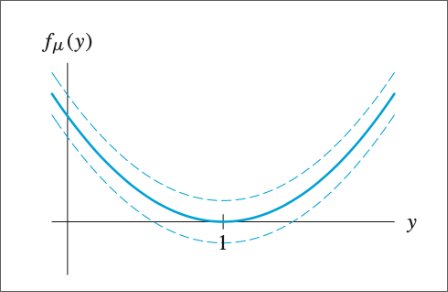
\includegraphics[width=50mm]{content/diffeq/images/bifurcation_0.png}
    % \caption{Graph of $f_\mu(y) = y^2 - 2y + \mu$ for $\mu < 1$, $\mu = 1$, and $\mu > 1$.}
\end{figure}
Figure: Graph of $f_\mu(y) = y^2 - 2y + \mu$ for $\mu < 1$, $\mu = 1$, and $\mu > 1$.

\begin{figure}[H]
    \centering
    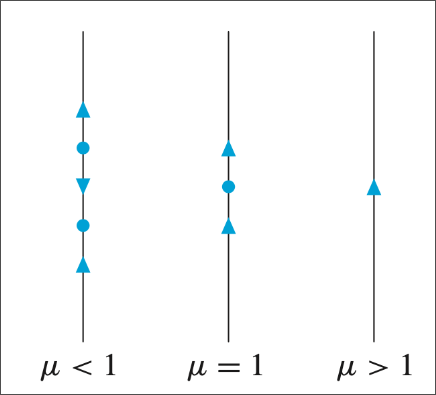
\includegraphics[width=50mm]{content/diffeq/images/bifurcation_1.png}
    % \caption{Corresponding phase portraits for $\frac{dy}{dx} = y^2 - 2y + \mu$.}
\end{figure}
Figure: Corresponding phase portraits for $\frac{dy}{dx} = y^2 - 2y + \mu$.

The typical way to visualize bifurcations is through \textit{bifurcation diagrams}. The parabola on the following figure is called a \textit{bifurcation line}.

\begin{figure}[H]
    \centering
    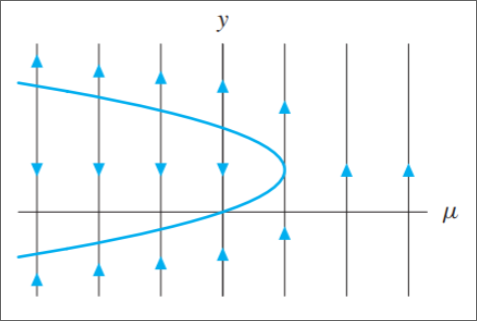
\includegraphics[width=50mm]{content/diffeq/images/bifurcation_2.png}
    % \caption{Bifurcation diagram for $\frac{dy}{dx} = y^2 - 2y + \mu$.}
\end{figure}
Figure: Bifurcation diagram for $\frac{dy}{dx} = y^2 - 2y + \mu$.

\subsection{Separable Equations}

\begin{definition}[Separable first-order ODE]
    An ODE is separable if it can be expressed as 
    \[
        \frac{dy}{dx} = g(x)h(y)
    \]
    where $g$ and $h$ are continuous.
\end{definition}

We can simplify the process of solving a separable equations by defining the following where $H(y)$ and $G(x)$ are antiderivatives of $\frac{1}{h(y)}$ and $g(x)$, respectively, and $c \in \Real$ is an arbitrary constant.

\[
    H(y) = G(x) + c
\]

which can then be expressed as

\[
    \int \frac{1}{h(y)} dy = \int g(x) dx
\]

\subsection{Implicitly-Defined Solutions}

Sometimes a separable equation can't be solved for $y$ explicitly. Let's define $F(x,y)$ as

\[
    F(x,y) \coloneq H(y) - G(x) - c
\]

so that

\[
    F(x,y) = 0
\]

The equation above implicitly defines $y$ as a function of $x$ only if it follows the \textit{Implicit Function Theorem} from Multivariable Calculus.

\begin{theorem}[Implicit Function Theorem]
    If $F$ is defined on a disc containing $(x_0, y_0)$, where

    \begin{enumerate}
        \item $F(x,y) = 0$
        \item $\frac{\partial^{}F}{\partial^{}x}$ and $\frac{\partial^{}F}{\partial^{}y}$ are continuous on the disc
        \item $\frac{\partial^{}F}{\partial^{}x} \ne 0$
    \end{enumerate}

    then the equation $F(x,y) = 0$ defines $y$ as a function of $x$ on some open set containing the point $(x_0, y_0)$.
\end{theorem}

\subsection{Singular Solutions}

\begin{definition}[Singular Solution]
    A solution is singular if it cannot be obtained by any choice of $c$ in the solution equation of the separable ODE.
\end{definition}

When either $h(y)$ or $g(x)$ are equal to $0$ inside a separable equation, then they would be valid solutions, but may not show up in the integration method for finding solutions as defined in the Separable Equations section. If that is the case, then those solutions are unique.

\subsection{Orthogonal Trajectories}

An \textit{orthogonal trajectory} of a family of curves is a curve that intersects each curve of the family orthogonally.

\begin{figure}[H]
    \centering
    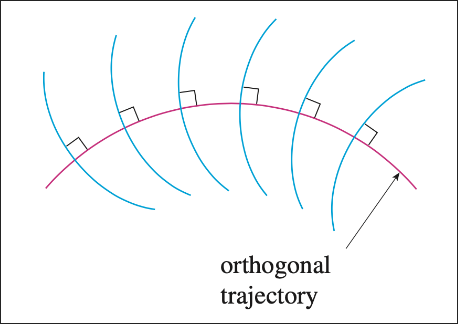
\includegraphics[width=50mm]{content/diffeq/images/orthogonal_0.png}
    % \caption{An example of an orthogonal trajectory.}
\end{figure}
Figure: An example of an orthogonal trajectory.

For example,

\[
    x^2 + y^2 = r^2
\]

and

\[
    y = mx
\]

are orthogonal trajectories of each other.

To find orthogonal trajectories of an equation in terms of $x$, $y$, and another constant variable:

\begin{enumerate}
    \item Take derivative of both sides in respect to $x$
    \item Solve for $\frac{dy}{dx}$ from previous equation
    \item Use the original equation to eliminate the constant and write an expression that only depends on $x$ and $y$
    \item The previous equation is a slope $m(x,y)$; find the orthogonal slope at point $(x,y)$
    \item Solve the differential equation $\frac{dy}{dx} = m(x,y)$ to find the family of orthogonal trajectories
\end{enumerate}

\subsection{Linear Equations}

\begin{definition}[Linear Equation]
    An equation is linear if it can be expressed in the from
    \[
        \frac{dy}{dx} = p(x)y + q(x)
    \]
    where $p,q : (a,b) \rightarrow \Real, -\infty \le a < b \ge \infty$ are continuous.
\end{definition}

If $q(x) = 0$, then the linear equation is called \textit{homogeneous}. If $p(x)$ is a constant, but not necessarily $q(x)$, it is called \textit{constant-coefficient}.

\subsection{Variation of Parameters}

If $y_h(x)$ is a solution of a homogeneous linear equation, then $cy_h(x)$ is also a solution of the same homogeneous equation. A general solution of a homogeneous linear equation is
\[
    y_h(x) = ce^{\int p(x)dx}
\]

A general solution of nonhomogeneous linear equation is
\[
    y(x) = ce^{\int p(x)dx} + e^{\int p(x)dx}\int e^{-\int p(x)dx}q(x)dx
\]

\subsection{Integrating Factors}

This can be simplified by defining
\[
    \mu(x) \coloneq e^{-\int p(x)dx}
\]
\[
    y(x) = \frac{1}{\mu(x)}\int \mu(x)q(x)dx
\]

\subsection{Singular Points}

If we represent a linear equation in the form
\[
    a_1(x)\frac{dy}{dx} + a_0(x)y = g(x)
\]
and divide both sides by $a_1(x)$, then $p$ and $q$ will be discontinuous when $a_1(x) = 0$. These points are called \textit{singular points}. These discontinuous points carry over to the final solution.

\subsection{Bernoulli's Equation}

An ODE in the from

\[
    \frac{dy}{dx} = p(x)y + f(x)y^n
\]

where $n \in \Real$, is called \textit{Bernoulli's equation}.

This equation is linear if $n = 0, 1$. By substituting $u = y^{1-n}$, the equation can be rewritten in a linear form as
\[
    \frac{du}{dx} = (1 - n)(p(x)u + q(x))
\]
where $n \ne 0,1$.

\subsection{Exact Equations}

An exact equation is a differential equation in the form
\[
    M(x, y) + N(x, y)\frac{dy}{dx} = 0
\]
where $M, N$ are continuously differentiable. They also represent partial derivatives of the potential function $\psi$

\[
    \psi_x + \psi_y\frac{dy}{dx} = 0
\]

where $\psi(x, y)$ is an existing \textit{potential function}, as seen in Multivariable Calculus. The equation is exact only if,
\begin{itemize}
    \item $\psi_{xy} = \psi_{yx}$
    \item Domain of functions above is open and topologically simply-connected (continuous)
\end{itemize}

So if the potential function exists, then the solution to the equation would be
\[
    \psi(x, y) = 0
\]

\subsection{Homogeneous Equations}

A real-valued function is \textit{homogeneous of degree} $\alpha$ if it can be rewritten in the form
\[
    f(tx, ty) = t^{\alpha}f(x, y)
\]
where $\alpha, t \in \Real$.

A first-order differential equation of the form
\[
    M(x, y) + N(x, y)\frac{dy}{dx} = 0
\]
is called \textit{homogeneous} if both $M$ and $N$ are homogeneous of the same degree. To solve it, simply remember the substitution
\[
    y = ux
\]

\subsection{$n$th-Order Linear Equations}

An \textit{nth-order differential equation} is in the form
\[
    a_n(x)\frac{d^n y}{dx^n} + a_{n-1}(x)\frac{d^{n-1} y}{dx^{n-1}} + \cdots + a_1(x)\frac{dy}{dx} + a_0(x)y = g(x)
\]
where the functions $a_i, g: (a, b) \to \Real$ are continuous.
An \textit{nth-order initial value problem} (IVP) is to find the solution of the equation above where $x_0$ on interval $I$ is subject to $n$ initial conditions
\[
    y(x_0) = y_0,\qquad y'(x_0) = y_1,\qquad \ldots,\qquad y^{n-1}(x_0) = y_{n-1}
\]

\begin{theorem}
    If $a_n(x) \ne 0$ on $I$ and $x_0 \in I$, then a solution $y$ of the $n$th-order IVP exists on $I$ and is unique.
\end{theorem}

\subsection{Boundary Value Problems}

A boundary value problem (BVP) is when a linear differential equation of order two or greater has the dependent variable $y$ or its derivatives specified at different points. E.g. $y(a) = y_0, y(b) = y_1$. Those values are called \textit{boundary conditions}. A solution to this BVP would satisfy the differential equation on $I$, whose graph passes through $(a, y_0)$ and $(b, y_1)$. Those boundary conditions can be often written as
\[
    \alpha_1y(a) + \beta_1y'(a) = \gamma_1,
\]
\[
    \alpha_2y(a) + \beta_2y'(a) = \gamma_2,
\]
where $\alpha_1, \alpha_2, \beta_1, \beta_2, \gamma_1, \gamma_2$ are arbitrary constants. Conclusions of the earlier defined theorem regarding IVP for $n$th-order equations does not apply to BVP.

\subsection{Homogeneous ($n$th-Order Linear) Equations}

An $n$th-order linear differential equation is homogeneous if $g(x)$ in
\[
    a_n(x)\frac{d^n y}{dx^n} + a_{n-1}(x)\frac{d^{n-1} y}{dx^{n-1}} + \cdots + a_1(x)\frac{dy}{dx} + a_0(x)y = g(x)
\]
is equal to zero. First the associated homogeneous equation has to be solved before solving the nonhomogeneous equation.

\subsection{Differential Operators}

The symbol $D$ is the \textit{differential operator}, where
\[
    D^n y = \frac{d^n y}{dx^n}.
\]

The \textit{n-th order differential operator} or \textit{polynomial operator} is
\[
    L = a_n(x)D^n + a_{n - 1}(x)D^{n - 1} + \cdots + a_1(x)D + a_0(x)
\]

Using $L$, $n$th-order linear equations can be written as
\[
    Ly = 0 \qquad \text{and} \qquad Ly = g(x)
\]

The operator is also linear so it has the property
\[
    L(c_1f(x) + c_2g(x)) = c_1Lf(x) + c_2Lg(x)
\]

\begin{theorem}[Superposition Principle for Homogeneous Linear Equations]
    Let $y_1, \ldots, y_k$ be solution of $Ly = 0$ on interval $I$. Then the linear combination
    \[
        y = c_1 y_1 + \cdots + c_k y_k
    \]
    where $c_i$ are constants, is also a solution of $Ly = 0$.
\end{theorem}
By this theorem, every homogeneous $n$th-order linear equation has a solution of $y = 0$.

\subsection{Linear Dependence and Independence}

\begin{definition}[Linear Dependence]
    A set of functions is \textit{linearly dependent} on interval $I$ if there exists constants $c_i$, not all zero, where
    \[
        c_1 f_1(c) + \cdots + c_n f_n(x) = 0
    \]
    for all $x$ in $I$. If the only constants for which the equation above is satisfied are
    \[
        c_1 = c_2 = \cdots = c_n = 0
    \]
    then the set is \textit{linearly independent}.
\end{definition}

\begin{definition}[Wronskian]
    Given that each function in $f_1, \ldots, f_n$ is at least $n - 1$ times differentiable, the determinant
    \[
        W(f_1, f_2, \ldots, f_n) = \begin{vmatrix}
            f_1 & f_2 & \cdots & f_n \\
            f_1' & f_2' & \cdots & f_n' \\
            \vdots & \vdots & & \vdots \\
            f_1^{(n - 1)} & f_2^{(n - 1)} & \cdots & f_n^{(n - 1)}
        \end{vmatrix}
    \]
    is called the \textit{Wronskian} of the functions.
\end{definition}

The set of solutions $y_1, y_2, \ldots, y_n$ on interval $I$ for a homogeneous equation is linearly independent only if $W(y_1, y_2, \ldots, y_n) \ne 0$ on $I$.

This linearly independent set of solutions is called the \textit{fundamental set of solutions} on the specified interval.

\begin{theorem}[Existence of a Fundamental Set]
    If functions $a_i$, $g$ are continuous on some common interval $I$, and $a_n(x) \ne 0$ on $I$, then there exists a fundamental set of solutions of the homogeneous linear $n$th-order differential equation.
\end{theorem}

Given that $y_1, y_2, \ldots, y_n$ is the fundamental set of solutions for the homogeneous equation on $I$, then its general solution is
\[
    y = c_1 y_1(x) + c_2 y_2(x) + \cdots + c_n y_n(x)
\]
where $c_i$ are arbitrary real constants.

Any function $y_p$, free of arbitrary parameters, that satisfies the nonhomogeneous equation, is said to be the \textit{particular solution} of the equation.

\begin{theorem}
    The general solution of the $n$th-order nonhomogeneous equation is of the form
    \[
        y(x) = y_p(x) + c_1 y_1(x) + c_2 y_2(x) + \cdots + c_n y_n(x)
    \]
    where $y_p$ is the particular solution and $y_1, \ldots, y_n$ are a fundamental set of solutions of the associated homogeneous equation.
\end{theorem}

\subsection{Reduction of Order}

Reduction of order is a method of substitution to reduce a homogeneous second order equation to a first order equation. This can be used to find a second nontrivial solution using the first and create a fundamental set of solutions.
\[
    y_2(x) = y_1(x) \int \frac{e^{-\int P(x)dx}}{y_1^2(x)}dx
\]
where the original equation is in the standard form
\[
    y'' + P(x)y' + Q(x)y = 0
\]

\subsection{Reduction of order for nonhomogeneous equations}

The equation
\[
    y_p(x) = y_1(x) \left[ \int \frac{e^{-\int P(x)dx}}{(y_1(x))^2} \left[ \int e^{\int P(x)dx} y_1(x) R(x)dx + c_1 \right] dx + c_2 \right]
\]
can be used to find the particular solution needed for general equation of the nonhomogeneous standard equation
\[
    y'' + P(x)y' + Q(x)y = R(x)
\]